\documentclass[12pt]{beamer}
\usepackage{../latex-sty/mypres}
\usepackage[utf8]{inputenc}
\usepackage[T2A]{fontenc}
\usepackage[russian]{babel}

\expandafter\def\expandafter\insertshorttitle\expandafter{%
  \insertshorttitle\hfill%
  \insertframenumber\,/\,\inserttotalframenumber}
\title[]{Условия оптимальности.\\Теория двойственности}
\author{Александр Катруца}
\institute{Московский физико-технический институт,\\
Факультет Управления и Прикладной Математики} 
\date{\today}

\begin{document}
\begin{frame}
\maketitle
\end{frame}

\begin{frame}{Напоминание}
\begin{itemize}
\item Выпуклые множества
\item Выпуклые функции
\item Критерии выпуклости
\item Операции, сохраняющие выпуклость
\end{itemize}
\end{frame}

\begin{frame}{Мотивация}

\begin{block}{Вопрос 0}
Когда существует решение оптимизационной задачи?
\end{block}

\begin{block}{Вопрос 1}
Как проверить, что точка является решением оптимизационной задачи? 
\end{block}

\begin{block}{Вопрос 2}
Из каких условий можно найти решение оптимизационной задачи?
\end{block}

\end{frame}

\begin{frame}{Существование решения}
\begin{block}{Теорема Вейерштрасса}
Пусть $X \subset R^n$ компактное множество и пусть $f(x)$ непрерывная функция на $X$. 
Тогда точка глобального минимума функции $f (x)$ на $X$ существует.
\end{block}

Эта теорема гарантирует, что решение подавляющего большинства разумных задач существует.
 
\end{frame}

\begin{frame}{Условия оптимальности}
\begin{block}{Определение}
Условием оптимальности будем называть некоторое выражение, выполнимость которого даёт необходимое и (или) достаточное условие экстремума. 
\end{block}
Классы задач:
\begin{itemize}
\item Общая задача минимизации
\item Задача безусловной минимизации
\item Задача минимизации с ограничениями типа равенств
\item Задача минимизации с ограничениями типа равенств и неравенств
\end{itemize}
\end{frame}

\begin{frame}{Общая задача минимизации}

\begin{block}{Задача}
\[
f(x) \rightarrow \min\limits_{{\color{red}{x \in X}}}
\]
\end{block}

\begin{block}{Критерий оптимальности}
Пусть $f(x)$ определена на множестве $X \subset \bbR^n$.
Тогда 
\begin{enumerate}
\item если $x^*$ точка минимума $f(x)$ на $X$, то $\partial_X f(x^*) \neq \emptyset$ и $0 \in \partial_X f(x^*)$
\item если для некоторой точки $x^* \in X$ существует субдифференциал $\partial_X f(x^*)$ и $0 \in \partial_X f(x^*)$, то $x^*$~--- точка минимума $f(x)$ на $X$.
\end{enumerate}
\end{block}
Какие недостатки у приведённого критерия?

\end{frame}

%\begin{frame}{Примеры}
%\begin{itemize}
%\item $\bx^{\T}\bx + \alpha \| \bx - 
%\bc \|_2 \rightarrow \min\limits_{\bx \in \bbR^n}$, $\alpha > 0$
%\item $\bx^{\T}\bx + \alpha \| \bc^{\T}\bx - 
%b \|_2 \rightarrow \min\limits_{\bx \in \bbR^n}$, $\alpha > 0$
%\item Ограничение на допустимое множество
%\begin{equation*}
%\begin{split}
%\vspace{-4mm}
%&(x + 2)^2 + |y + 3| \rightarrow \min\limits_{(x, y) \in \bbR^2}\\
%\text{s.t. }& 8 + 2x - y \leq 0
%\end{split}
%\end{equation*}
%\end{itemize}
%\end{frame}

\begin{frame}{Задача безусловной минимизации}
Задача: $f(x) \rightarrow \min\limits_{\color{red}{x \in \bbR^n}}$.

\begin{block}{Критерий оптимальности для выпуклых функций}
Пусть $f(x)$ выпуклая функция на $\bbR^n$. 
Тогда точка $x^*$ решение задачи безусловной минимизации $\Leftrightarrow$ $0 \in \partial f(x^*)$.
\end{block}

\begin{block}{Следствие}
Если $f(x)$ выпукла и дифференцируема на $\bbR^n$.
Тогда точка $x^*$ решение задачи безусловной минимизации $\Leftrightarrow$ $\nabla f(x^*) = 0$.
\end{block}

\begin{block}{Достаточное условие для невыпуклых функций}
Пусть $f$ дважды дифференцируема на $\bbR^n$ и $x^*$ такая что $\nabla f(x^*) = 0$. 
Тогда если $\nabla^2 f(x^*) \succ 0$, то $x^*$ точка строгого локального минимума $f(x)$ на $\bbR^n$.  
\end{block}

\end{frame}

%\begin{frame}{Примеры}
%\begin{itemize}
%\item $x_1e^{x_1} - (1 + e^{x_2})\cos x_2 \rightarrow \min$
%\item Функция Розенброка: $(1 - x_1)^2 + \alpha \sum\limits_{i = 2}^n (x_i - x_{i-1})^2 \rightarrow \min$, $\alpha > 0$
%\item $x^2_1 + x^2_2 - x_1x_2 + e^{x_1 + x_2} \rightarrow \min$
%\end{itemize}
%\end{frame}

\begin{frame}{{\small Задача минимизации с ограничениями типа равенств}}

\begin{block}{Задача}
\vspace{-3mm}
\begin{equation*}
\begin{split}
& f(x) \rightarrow \min\limits_{x \in \bbR^n} \\
\text{s.t. } & g_i(x) = 0, \; i = 1,\ldots, m 
\end{split}
\end{equation*}
\end{block}

\begin{block}{Лагранжиан}
\vspace{-2mm}
\begin{equation*}
L(x, \blambda) = f(x) + \sum\limits_{i=1}^m\lambda_i g_i(x)
\end{equation*}
\end{block}

\begin{block}{Критерий оптимальности}
Пусть $f(x)$ и $g_i(x)$ дважды дифференцируемы в точке $x^*$ и непрерывно дифференцируемы в некоторой окрестности $x^*$.
Пусть также $\nabla_x L(x^*, \blambda) = 0$.
Тогда если $\bh^{\T}\nabla^2 L(x^*, \blambda)\bh > 0$, где $\bh \in T(\bx^*|G)$~--- касательный конус, то $x^*$~--- точка локального минимума.
\end{block}

\end{frame}

\begin{frame}{Возможные варианты}
\begin{figure}
\centering
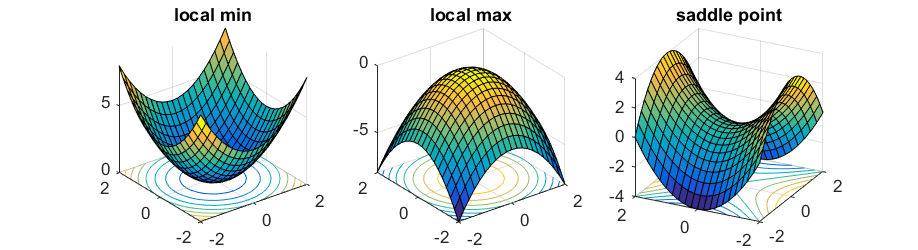
\includegraphics[scale=0.5]{minmaxsaddle.png}
\caption{Рисунок взят из блога \url{http://www.offconvex.org/2016/03/22/saddlepoints/}}
\end{figure}
\end{frame}

%\begin{frame}{Примеры}
%\begin{itemize}
%\item $\sum\limits_{i=1}^n\alpha_i x^4_i \rightarrow \extr\limits_{\bx \in G}$, $G = \{\bx \in \bbR^n \; | \; \bc^{\T}\bx = 1 \}$, $\alpha_i > 0,\; c_i > 0$
%\item $x_1 + 4x_2 + 9x_3 \rightarrow \extr\limits_{\bx \in G}, \; G = \left \{ \frac{1}{x_1} + \frac{1}{x_2} + \frac{1}{x_3} = 1 \right\}$
%\item Примеры из задачника по матану на метод множителей Лагранжа
%\end{itemize}
%\end{frame}

\begin{frame}{{Задача минимизации с ограничениями типа равенств и неравенств}}

\begin{block}{Задача}
\vspace{-5mm}
\begin{equation*}
\begin{split}
& \min\limits_{x \in \bbR^n} f(x)\\
\text{s.t. } & g_i(x) = 0, \; i = 1,\ldots,m\\
& h_j(x) \leq 0, \; j = 1,\ldots, p
\end{split}
\end{equation*}
\end{block}

\begin{block}{Лагранжиан}
\begin{equation*}
L(x, \blambda, \bmu) = f(x) + \sum\limits_{i=1}^m\lambda_i g_i(x) + \sum\limits_{j=1}^p \mu_j h_j(x)
\end{equation*}
\end{block}
\end{frame}

\begin{frame}{Условия оптимальности}
\begin{block}{Необходимое условие (Каруша-Куна-Такера)}
Пусть $x^*$ решение задачи математического программирования, и функции $f, h_j, g_i$ дифференцирумы. 
Тогда найдутся такие $\bmu^*$ и $\blambda^*$, что выполнены следующие условия:
\begin{itemize}
\item $g_i(x^*) = 0$
\item $h_j(x^*) \leq 0$
\item $ \mu^*_j \geq 0$
\item $\mu^*_jh_j(x^*) = 0$
\item $\nabla_x L(x^*, \blambda^*, \bmu^*) = 0$
\end{itemize}
\end{block}
Если задача выпуклая, то это же условие является достаточным.
\end{frame}

\begin{frame}{Условия оптимальности (cont'd)}
\small
Если задача невыпуклая, то
\begin{block}{Достаточное условие первого порядка}
\small
Если для стационарной точки $(x^*, \blambda^*, \bmu^*)$ число активных неравенств $|J|$ такое что $n = m + |J|$ и $\mu_j > 0, \; j \in J$, то эта точка является точкой минимума.
\end{block}

\begin{block}{Достаточное условие второго порядка}
\small
Если в задаче математического программирования число активных ограничений меньше размерности задачи, то точка $x^*$ яляется решением задачи, если выполнены условия
\vspace{-3mm}
\[
\bz^{\T}\nabla_{xx}^2 L(x^*)\bz > 0
\vspace{-3mm}
\] 
для 
\vspace{-4mm}
\begin{itemize}
\item $\bz \neq 0$ и $\nabla g^{\T}_i(x^*)\bz = 0$
\vspace{-3mm}
\item при $j \in J$ и $\mu_j > 0$, $\nabla h^{\T}_j(x^*) \bz = 0$
\vspace{-3mm}
\item при $j \in J$ и $\mu_j = 0$, $\nabla h^{\T}_j(x^*) \bz \leq 0$
\end{itemize}
\end{block}

\end{frame}

%\begin{frame}{Примеры}
%\begin{itemize}
%\small
%\item Пример 1
%\vspace{-5mm}
%\begin{equation*}
%\begin{split}
%& \extr (x_1 - 3)(x_2 - 2)\\
%\text{s.t. } & x_1 + 2x_2 = 4\\
%& x^2_1 + x^2_2 \leq 5\\
%& x_1 \geq 0, \; x_2 \geq 0 
%\end{split}
%\end{equation*} 
%\vspace{-5mm}
%\item Пример 2
%\vspace{-5mm}
%\begin{equation*}
%\begin{split}
%& \extr \sum\limits_{i=1}^n \frac{c_i}{x_i}\\
%\text{s.t. } & \sum\limits_{i=1}^n a_ix_i \leq b\\
%& x_i > 0, \; b > 0, \; c_i > 0, \; a_i > 0
%\end{split}
%\end{equation*}
%\vspace{-4mm}
%\item Пример 3
%\vspace{-3mm}
%\begin{equation*}
%\begin{split}
%& \extr (x_1x_3 - 2x_2)\\
%\text{s.t. } & 2x_1 - x_2 - 3x_3 \leq 10\\
%& 3x_1 + 2x_2 + x_3 = 6\\
%& x_2 \geq 0
%\end{split}
%\end{equation*}
%\end{itemize}
%\end{frame}

\begin{frame}{Двойственность: обозначения}
\small
\begin{block}{Задача}
\vspace{-5mm}
\begin{equation*}
\begin{split}
& \min\limits_{x \in \mathcal{D}} f(x) = p^*\\
\text{s.t. } & g_i(x) = 0, \; i = 1,\ldots,m\\
& h_j(x) \leq 0, \; j = 1,\ldots, p
\end{split}
\end{equation*}
\end{block}

\begin{block}{Лагранжиан}
\vspace{-2mm}
\begin{equation*}
L(x, \blambda, \bmu) = f(x) + \sum\limits_{i=1}^m\lambda_i g_i(x) + \sum\limits_{j=1}^p \mu_j h_j(x)
\vspace{-2mm}
\end{equation*}
\end{block}

\begin{block}{Двойственные переменные}
Вектора $\bmu$ и $\blambda$ называются двойственными переменными.
\end{block}

\begin{block}{Двойственная функция}
Функция $g(\bmu, \blambda) = \inf\limits_{x\in \mathcal{D}} L(x, \blambda, \bmu)$ называется двойственной функцией Лагранжа.
\end{block}

\end{frame}

\begin{frame}{Свойства двойственной функции}
\small
\begin{block}{Вогнутость}
Двойственная функция является {\color{red}{вогнутой}} как инфимум аффинных функций по $(\bmu, \blambda)$ вне зависимости от того, является ли исходная задача выпуклой.
\end{block}

\begin{block}{Нижняя граница}
Для любого $\blambda$ и для $\bmu \geq 0$ выполнено $g(\bmu, \blambda) \leq p^*$.
\end{block}

\begin{block}{Двойственная задача}
\vspace{-5mm}
\begin{equation*}
\begin{split}
& \max g(\bmu, \blambda) = d^*\\
\text{s.t. } & \bmu \geq 0
\end{split}
\end{equation*}
\end{block}

\begin{block}{Зачем?}
\begin{itemize}
\vspace{-2mm}
\item Двойственная задача выпукла независимо от того, выпукла ли прямая
\vspace{-3mm}
\item Нижняя оценка \textbf{может} достигаться
\end{itemize}
\end{block}
\end{frame}

%\begin{frame}{Связь с сопряжённой функцией}
%Рассмотрим задачу
%\begin{equation*}
%\begin{split}
%&\min f_0(x) \\
%\text{s.t. } & \bA\bx \leq \mathbf{b}\\
%& \bC\bx = \bd
%\end{split}
%\end{equation*}
%Тогда
%\begin{equation*}
%\begin{split}
%& g(\blambda, \bmu) = \inf_{\bx} (f_0(\bx) + \blambda^{\T}(\bA\bx - \mathbf{b}) + \bmu^{\T}(\bC\bx - \bd)) = \\
%& - \mathbf{b}^{\T}\blambda - \bmu^{\T}\bd + \inf_{\bx}(f_0(\bx) + (\bA^{\T}\blambda + \bC^{\T}\bmu)^{\T}\bx) = \\
%& - \mathbf{b}^{\T}\blambda - \bmu^{\T}\bd - f_0^*(-\bA^{\T}\blambda - \bC^{\T}\bmu)
%\end{split}
%\end{equation*}
%Области определений двойственной и сопряжённой функций связаны:
%\[
%\text{dom } g = \{ (\blambda, \bmu) \; | \; -\bA^{\T}\blambda - \bC^{\T}\bmu \in \text{dom } f^*_0 \}
%\] 
%\end{frame}

\begin{frame}{Примеры}
Найти двойственную функцию:
\begin{itemize}
\item Решение СЛУ минимальной нормы 
\vspace{-3mm}
\begin{equation*}
\begin{split}
& \min \| \bx\|^2_2\\
\text{s.t. } & \bA\bx = \mathbf{b}
\end{split}
\end{equation*}
\item Линейное программирование
\vspace{-3mm}
\begin{equation*}
\begin{split}
& \min \bc^{\T}\bx\\
\text{s.t. } & \bA\bx = \mathbf{b}\\
& \bx \geq 0
\end{split}
\end{equation*}
\item Задача разбиения
\vspace{-3mm}
\begin{equation*}
\begin{split}
& \min \bx^{\T}\bW\bx\\
\text{s.t. } & x^2_i = 1, \; i = 1,\ldots,n
\end{split}
\end{equation*}
\end{itemize}
\end{frame}

\begin{frame}{Слабая и сильная двойственность}
\small
\begin{block}{Определение}
Оптимальные значения целевой функции в прямой и двойственной задаче связаны соотношением 
\vspace{-3mm}
\[
d^* \leq p^*.
\vspace{-4mm}
\]
Если $d^* < p^*$, то свойство называют слабой двойственностью.
Если $d^* = p^*$, то~--- сильной двойственностью.
\end{block}

\begin{block}{Замечание}
Слабая двойственность есть всегда по построению двойственной задачи.
\end{block}

\begin{block}{Вопросы}
\begin{itemize}
\item При каких условиях выполняется сильная двойственность?
\vspace{-7mm}
\item Как использовать двойственность для проверки оптимальности?
\end{itemize}
\end{block}
\end{frame}

\begin{frame}{Критерий субоптимальности}
По построению $p^* \geq g(\blambda, \bmu)$, поэтому $f_0(x) - p^* \leq f_0(x) - g(\blambda, \bmu) = \varepsilon$.
\begin{block}{Определение}
Разность $f_0(x) - g(\blambda, \bmu)$ называется \emph{двойственным зазором} и является оценкой сверху для разности текущего и оптимального значения функции.
\end{block}
Способы использования:
\begin{itemize}
\item критерий остановки в итерационном процессе
\item теоретическая оценка сходимости алгоритма
\item проверка оптимальности данной точки
\end{itemize}
\end{frame}

\begin{frame}{Условия Слейтера}
\begin{block}{Теорема}
Если задача выпуклая и существует $x$, лежащий внутри допустимой области, т.е. ограничения типа неравенств выполнены как строгие неравенства, то выполнено свойство сильной двойственности.
\end{block}

\begin{itemize}
\item Решение СЛАУ наименьшей нормы
\item Линейное программирование
\item Квадратичное программирование с квадратичными огранчиениями
\item Невыпуклая задача с сильной двойственностью
\end{itemize}
\end{frame}

%\begin{frame}{Геометрическая интерпретация}
%\begin{center}
%$\min\limits_{x} f_0(x), \text{ where } f_1(x) \leq 0.$
%\end{center}
%$
%g(\lambda) = \inf\limits_{(u, t) \in \mathcal{G}} (t + \lambda u) \qquad \mathcal{G} = \{ (f_1(x), f_0(x)) \; | \; x \in \mathcal{D} \}
%$
%
%\begin{figure}
%\centering
%\includegraphics[scale=0.3]{dual_geometry.png}
%\end{figure}
%\begin{itemize}
%\item $\lambda = 0$
%\item $\lambda^*$~--- оптимальное значение
%\item $\lambda > \lambda^*$
%\end{itemize}
%\end{frame}

\begin{frame}{Условия дополняющей нежёсткости}
Пусть $\bx^*$ и $(\bmu^*, \blambda^*)$ решения прямой и двойственной задачи. То есть
\begin{equation*}
\begin{split}
& f(\bx^*) = g(\bmu^*, \blambda^*) = \inf\limits_{\bx} L(\bx, \blambda, \bmu) \leq \\
& f(\bx^*) + \sum\limits_{i=1}^m\lambda^*_i g_i(\bx^*) + \sum\limits_{j=1}^p \mu^*_j h_j(\bx^*) \leq\\
& f(\bx^*), \qquad \bmu \geq 0 
\end{split}
\end{equation*}

\begin{block}{Условия дополняющей нежёсткости}
\[
\mu^*_j h_j(\bx^*) = 0, \qquad j = 1,\ldots,p 
\]
Для каждого неравенства
\begin{itemize}
\item либо множитель Лагранжа равен нулю
\item либо оно активно.
\end{itemize} 
\end{block}
\end{frame}

\begin{frame}{Условия Каруша-Куна-Таккера}
Hеобходимые условия~ККТ: 
\begin{enumerate}
\item $g_i(x^*) = 0$~--- допустимость в прямой задаче
\item $h_j(x^*) \leq 0$~--- допустимость в прямой задаче
\item $ \mu^*_j \geq 0$~--- допустимость в двойственной задаче
\item $\mu^*_jh_j(x^*) = 0$~--- условие дополняющей нежёсткости
\item $\nabla_x L(x^*, \blambda^*, \bmu^*) = 0$~--- стационарность лагранжиана по прямым переменным
\end{enumerate}
Пример $(\bP \in \mathcal{S}^n_+)$
\begin{equation*}
\begin{split}
& \min\limits_{\bx \in \bbR^n} \frac{1}{2}\bx^{\T}\bP\bx + \bq^{\T}\bx + r\\
\text{s.t. } & \bA\bx = \mathbf{b}
\end{split}
\end{equation*}
\end{frame}

\begin{frame}{Механическая интерпретация}
\begin{figure}
\centering
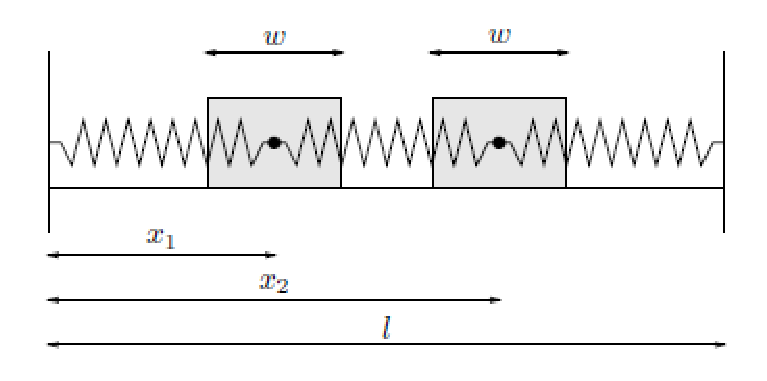
\includegraphics[scale=0.5]{kkt_mechanics.eps}
\end{figure}
Поиск устойчивого положения системы:
\begin{equation*}
\begin{split}
& \min_{\bx \in \bbR^3} \frac{1}{2}k_1x_1^2 + \frac{1}{2}k_2(x_2 - x_1)^2 + \frac{1}{2}k_3 (l - x_2)^2\\
\text{s.t. } & \frac{w}{2} - x_1 \leq 0\\
& w + x_1 - x_2 \leq 0\\
& \frac{w}{2} - l + x_2 \leq 0
\end{split}
\end{equation*}

\end{frame}

\begin{frame}{Примеры}
\footnotesize
\begin{itemize}
\item Орицательная энтропия при линейных ограничениях
\vspace{-5mm}
\begin{equation*}
\begin{split}
& \min\limits_{\bx \in \bbR^n} \sum\limits_{i=1}^n x_i \log x_i\\
\text{s.t. } & \bA\bx \leq \mathbf{b}\\
& \mathbf{1}^{\T}\bx = 1
\end{split}
\end{equation*} 
\item Сформулировать двойственную задачу и по её решению найти решение прямой задачи:
\begin{equation*}
\begin{split}
& \min \frac{1}{2}x^2 + 2y^2 + \frac{1}{2}z^2 + x + y + 2z\\
\text{s.t. } & x+2y+z = 4
\end{split}
\end{equation*}
\item Релаксация Лагранжа для задачи бинарного линейного программирования:
\begin{equation*}
\begin{split}
&\min\limits_{\bx \in \bbR^n} \bc^{\T}\bx\\
\text{s.t. } & \bA \bx \leq \mathbf{b}\\
& x_i \in \{0,1 \}, \quad i = 1,\ldots,n
\end{split}
\end{equation*}
\end{itemize}
\end{frame}

\begin{frame}{Резюме}
\begin{itemize}
\item Существование решения оптимизационной задачи 
\item Условия оптимальности для
\begin{itemize}
\item общей задачи оптимизации
\item задачи безусловной оптимизации
\item задачи оптимизации с ограничениями типа равенств
\item задачи оптимизации с ограничениями типа равенств и неравенств
\end{itemize}
\item Двойственая задача: что это такое и зачем оно надо?
\item Сильная и слабая двойственность
\item Условия Слейтера
\end{itemize}
\end{frame}
\end{document}